\section{Overview of Numerical Methods}\label{sec.overview}

%---------------------------------------------------------------------------%
\subsection{N-body dynamics}\label{sec.ov.nbody}
fft + multigrid


There are multiple methods to compute the gravitational potential 
(which is an elliptic equation in the Newtonian limit) in a structured 
AMR framework.  One way would be to model the dark matter (or other
collisionless particle-like objects, such as stars) as a second fluid 
in addition to the baryonic fluid and solve the collisionless
Boltzmann equation, which follows the evolution of the fluid density in
six-dimensional phase space.  However, this is computationally prohibitive 
owing to the large dimensionality of the problem, making this approach 
unappealing for the cosmological AMR code.

Instead, \enzo\ uses a particle-mesh N-body method to calculate 
the dynamics of collisionless systems \citep{Hockney88}.  This method 
follows trajectories 
of a representative sample of individual particles and is much more 
efficient than a direct solution of the Boltzmann equation in most 
astrophysical situations. 
The gravitational potential is computed by solving the elliptic 
Poisson's equation (Eq.~\ref{eq:potential}).



These equations are finite-differenced and for simplicity are solved with the
same timestep as the hydrodynamic equations, as discussed in 
Section~\ref{sec.ov.amr}.
The dark matter particles are distributed onto the grids
using the cloud-in-cell (CIC) interpolation technique to form a spatially
discretized density field (analogous to the baryon densities used to calculate
the equations of hydrodynamics).  After sampling dark matter density onto the
grid and adding baryon density if it exists (to get the total matter density
in each cell), the gravitational potential is calculated on the periodic root
grid using a fast Fourier transform.  In order to calculate more accurate
potentials on subgrids, \enzo\ re-samples the dark matter density onto
individual subgrids using the same CIC method as on the root grid, but at
higher spatial resolution (and again adding baryon densities if applicable).
Boundary conditions are then interpolated from the potential values on the
parent grid (with adjacent grid patches on a given level communicating to
ensure that their boundary values are the same), and then a multigrid
relaxation technique is used to calculate the gravitational potential at every
point within a subgrid.  Forces are computed on the mesh by
finite-differencing potential values and are then interpolated to the particle
positions, where they are used to update the particle's position and velocity
information.  Potentials on child grids are computed recursively and particle
positions are updated using the same timestep as in the hydrodynamic
equations.  Particles are stored in the most highly refined grid patch at the
point in space where they exist, and particles which move out of a subgrid
patch are sent to the grid patch covering the adjacent volume with the finest
spatial resolution, which may be of the same spatial resolution, coarser, or finer
than the grid patch that the particles are moved from.  This takes place in a
communication process at the end of each timestep on a level.

At this point it is useful to emphasize that the effective force
resolution of an adaptive particle-mesh calculation is approximately twice
as coarse as the grid spacing at a given level of resolution.  The 
potential is solved in each grid cell;
however, the quantity of interest, namely the acceleration, is the gradient
of the potential, and hence two potential values are required to calculate
this.  In addition, it should be noted that the adaptive particle-mesh
technique described here is very memory intensive: in order to ensure reasonably 
accurate force resolution at grid edges the multigrid relaxation
method used in the code requires a layer of ghost zones which is very deep --
typically 6 cells in every direction around the edge of a grid patch.  This greatly
adds to the memory requirements of the simulation, particularly because subgrids
are typically small (on the order of $12^3 - 16^3$ real cells for a standard 
cosmological calculation) and ghost zones can dominate the memory and computational 
requirements of the code.


%---------------------------------------------------------------------------%
\subsection{Hydrodynamics}\label{sec.ov.hydro}

\subsubsection{The PPM hydro method}\label{sec.ov.hydro.ppm}

\dcc{Removed ``things to do'' list.  Mention ppm-lr and ppm-de, and
  that ppm-de is preferred.  Briefly describe ppm-de itself.}

The primary hydrodynamic method used in \enzo\ is based on the
piecewise parabolic method (PPM) of
\citet{1984JCoPh..54..174C}, which has been
modified for the study of cosmological fluid flows.  
\citet{1984JCoPh..54..174C} describe two variants on this method: a
Lagrangian Remap variant and a Direct Eulerian variant.  Both have
been adapted for \enzo, and the Lagrangian Remap 
variant is described in \citet{1995CoPhC..89..149B}.  Because of its
conservative formulation, however, the Direct Eulerian variant is
preferred for \enzo\ AMR simulations.  We will describe the Direct
Eulerian (PPM-DE) variant and its additions briefly here, and in
further depth in Appendix \ref{app.ppm} 


PPM is an explicit, higher order-accurate version of
Godunov's method for ideal gas dynamics with third order-accurate piecewise parabolic
monotonic interpolation and a nonlinear Riemann solver for shock
capturing.  It advances the hydrodynamic equations in the following
steps:
\begin{enumerate}
 \item Construct monotonic parabolic interpolation of cell average
 data, for each fluid quantity.
 \item Compute interface states by averaging the parabola for over the domain of dependence for
 each interface
 \item Use interface data to solve the Riemann problem.
 \item Difference the interface fluxes to update the cell average quantities.
\end{enumerate}
It does an excellent job of capturing strong shocks in at
most two cells.  Multidimensional schemes are built up by directional
splitting and produce a method that is formally second order-accurate
in space and time which explicitly conserves mass, linear momentum, and energy.  

To use the above algorithm for cosmological simulations, the
conservation laws for fluid mass, momentum and energy 
density are written in comoving coordinates for a
Friedman-Robertson-Walker space-time, as described previously 
in Equations~\ref{enzoconserve} 
through~\ref{enzoenergy}.  Both the conservation laws and
the Riemann solver are modified to include gravity, which is solved
using an adaptive particle-mesh (PM) technique (see Section~\ref{sec.ov.nbody}).  
The terms due to cosmological expansion, as well as primordial chemistry and
radiative heating and cooling, are solved in a separate step because they have
different numerical behavior, and therefore must be treated differently to ensure
stability.  Note that unlike the \zeus\ hydro scheme, PPM does not need to use 
artificial viscosity to resolve shocks.

The system of equations described above works well for systems with
relatively low Mach numbers, as long as these systems are well resolved.  
However, cosmology is replete with situations where there are bulk hypersonic
flows.  In these situations, the ratio of kinetic to thermal energy can be
very high -- in some situations up to $10^6 - 10^8$.  This implies that the
thermal energy is an extremely tiny fraction of the kinetic energy, which can 
cause numerical problems when one is interested in just the thermal energy of the gas, since
 Equation~\ref{enzoenergy} solves for the total energy.  In this system of
equations, the
 thermal energy $E_{therm}$ is calculated as $E - E_{kin}$, 
where E is the total specific energy as
calculated in equation~\ref{enzoenergy} and $E_{kin}$ is the specific kinetic energy,
$0.5 \myvec{v}_b^2$.  
In hypersonic flows $E$ and $E_{kin}$ are nearly the same, and any 
number calculated as 
the difference of these is going to be strongly affected by numerical error.  To 
avoid this problem, \enzo\ also solves the internal energy equation in
comoving coordinates:

\begin{equation}
\frac{\partial e}{\partial t} + \frac{1}{a} \myvec{v}_b \cdot \grad e = 
- \frac{3(\gamma-1)\dot{a}}{a}e - \frac{p}{a \rho} \div \myvec{v}_b
\label{enzointenergy}
\end{equation}

In this equation $e$ is the internal energy (defined as $P/\rho (\gamma-1)$ and the other terms are as described
previously.  The code still conserves total energy ($E$) as well.  In order
to maintain consistency, both equations are solved at all times in all cells,
with the equation for the total energy (eqtn.~\ref{enzoenergy}) being used
for hydrodynamics routines and the internal energy $e$ being used when 
temperature is required.  When pressure is required for dynamic purposes,
the total energy is used if the ratio of thermal energy to total energy
is less than some threshold value $\eta$, and the internal energy is used
for values of the ratio larger than $\eta$.  A typical value of this parameter
is $10^{-3}$.  This \emph{dual energy formulation} ensures that the
method produces the correct entropy jump at strong shocks and also
yields accurate pressures and temperatures in cosmological hypersonic
flows.


\subsubsection{The Zeus hydro method}\label{sec.ov.hydro.zeus}


As a check on PPM, \enzo\ also includes an implementation of the
finite-difference hydrodynamic algorithm employed in the compressible 
magnetohydrodynamics code `\zeus'
\citep{Stone92a, Stone92b}.  Fluid transport is solved on a Cartesian
grid using the upwind, monotonic advection scheme of \citet{1977JCoPh..23..276V} 
within a multistep 
(operator split) solution procedure which is fully explicit in time.  
This method is formally second order-accurate in space but 
first order-accurate in time.  It is important to note that 
this method conserves internal energy
rather than total energy, so the ``dual energy
formulation'' discussed in Section~\ref{sec.ov.hydro.ppm} is unnecessary.
 

Operator split methods break
the solution of the hydrodynamic equations into parts, with each part
representing a single term in the equations.  Each part is evaluated
successively using the results preceding it.  The individual parts of
the solution are grouped into two steps, called the \emph{source} and
\emph{transport} steps.

The \zeus\ method uses a von Neumann-Richtmeyer artificial viscosity 
to smooth shock discontinuities that may
appear in fluid flows and can cause a break-down of finite-difference
equations.  The artificial viscosity term is added in the source terms
as
\begin{eqnarray}
\rho \frac{\partial\textbf{v}}{\partial t} &=& - \grad p - \rho \grad \phi 
- \div \textbf{Q} \\
\frac{\partial e}{\partial t} &=& -p \div \textbf{v} - \textbf{Q} : \grad \textbf{v}, 
\end{eqnarray}
where \textbf{v} is the baryon velocity, $\rho$ is the mass density,
$p$ is the pressure, $e$ is the internal energy density of the gas and \textbf{Q}
is the artificial viscosity stress tensor, such that:

\begin{eqnarray}
Q_{ii} = \left\{ \begin{array}{ll}
Q_{\rm AV} \rho_b  (a \Delta v_{i} + \dot{a} \Delta x_i)^2, 
& \textrm{for $a \Delta v_{i} + \dot{a} \Delta x_i < 0$}  \\
0 & \textrm{otherwise}\\
\end{array} \right. 
\end{eqnarray}
and
\begin{equation}
Q_{ij} = 0  \;\;\;{\rm for}\;\; i \ne j .
\end{equation}

$\Delta x_i$ and $\Delta v_{i}$ refer to the comoving 
width of the grid cell
along the $i$-th axis and the corresponding difference in gas
peculiar velocities across the grid cell, respectively, and $a$ is the
cosmological scale factor.  $Q_{\rm AV}$ is a constant with a typical
value of 2. We refer the interested reader to \citet{1994ApJ...429..434A} for more details.

The limitation of a technique that uses an artificial viscosity is that,
while the correct Rankine-Hugoniot jump conditions are achieved,
shocks are broadened over 6-8 mesh cells and are thus not treated as true
discontinuities. This may cause unphysical pre-heating of gas upstream
of the shock wave, as discussed in \citet{1994ApJ...429..434A}.

%---------------------------------------------------------------------------%
\subsection{Chemistry, radiation and cooling}
\label{sec.ov.chem}

\red{
As this stands it is the methods that I (brian) use, so I don't really emphasize
either the tabular cooling functions or the various radiation background options.
Add more discussion of this, point towards appendix.
}

Though the equations of hydrodynamics described above are a closed system,
they are still missing a crucial piece of physics: radiative heating and cooling.
Radiative cooling is extremely important in many astrophysical situations, as is 
the heating of gas from some sort of radiation background.  \enzo\ has a very simple
Sutherland and Dopita equilibrium cooling function \citep{1993ApJS...88..253S} 
implemented, which uses a
cooling table assuming a fixed metallicity of $Z = 0.3 Z_\odot$, and also a
nonequilibrium heating/cooling model that assumes gas of primordial composition exposed to a
uniform metagalactic ultraviolet (UV) background that varies with time \citep{1996ApJS..105...19K}.  

The simulations discussed in this thesis almost exclusively use the nonequilibrium
routines, described in great detail by Abel et al. and Anninos et al.  
\citep{abel97,anninos97} and summarized in Appendix~\ref{app:chemistry}. These 
routines follow the non-equilibrium chemistry of a 
gas of primordial composition with 9 total species:  
$H$, $H^+$, $He$, $He^+$, $He^{++}$, $H^-$, $H_2^+$, $H_2$, and $e^-$.  The code also calculates 
radiative heating and cooling, following atomic line excitation, recombination,
collisional excitation, free-free transitions, molecular line excitations, and Compton
scattering of the cosmic microwave background, as well as any of
approximately a dozen different models for a metagalactic UV background that heat
the gas via photoionization and photodissociation. 
The multispecies rate equations are solved out of
equilibrium to properly model situations where, e.g., the cooling rate of the gas
is much shorter than the hydrogen recombination time.  The effect of this nonequilibrium
cooling is to leave behind a much larger fraction of residual free electrons than one would
expect if the assumption of equilibrium were being made.  The practical effect of this
is that more $H^-$ is formed, which subsequently produces hydrogen molecules.  If large
amounts of $H_2$ is formed it can greatly increase the cooling rate of primordial gas
at relatively low temperatures ($T \leq 10^4$ K).  This can efficiently cool the gas 
to approximately $200$ K, which significantly reduces the Jeans mass of the gas.  Correct
modeling of the formation of molecular hydrogen is crucial to the study of star formation
in a primordial gas.

A total of 9 kinetic equations are solved, including 29 kinetic and radiative 
processes, for the 9 species mentioned above.  See Table~\ref{table.collisional} 
for the collisional processes and Table~\ref{table.radiative} for the 
radiative processes solved.

%---------------- table of collisional processes

\begin{table}
\begin{center}
{\bfseries Collisional Processes}\\[1ex]
\begin{tabular}{llllllll}
(1) & H & + & e$^-$ & $\rightarrow$ & H$^+$ &+& 2e$^-$ \\
(2) & H$^+$ &+ &e$^-$ & $\rightarrow$ & H &+ &$\gamma$ \\
(3) & He &+& e$^-$ & $\rightarrow$ & He$^+$ &+& 2e$^-$  \\
(4) & He$^+$ &+& e$^-$ & $\rightarrow$ & He &+ &$\gamma$  \\
(5) & He$^{+}$ &+& e$^-$ & $\rightarrow$ & He$^{++}$ &+& 2$e^-$  \\
(6) & He$^{++}$ &+& e$^-$ & $\rightarrow$ & He$^+$ &+& $\gamma$ \\
(7) & H &+& e$^-$ &$\rightarrow$& H$^-$ &+& $\gamma$  \\
(8) & H$^-$ &+& H &$\rightarrow$ & H$_2$ & +& e$^-$ \\
(9) & H &+ &H$^+$ &$\rightarrow$ &H$_2^+$ &+ &$\gamma$ \\
(10) & H$_2^+$ &+ &H &$\rightarrow$ &$H_2$ &+ &$H^+$ \\
(11) & H$_2$ &+ &H$^+$ &$\rightarrow$ &H$_2^+$ & +& H \\
(12) & H$_2$ &+ &e$^-$ & $\rightarrow$ & 2H & + & e$^-$  \\
(13) & H$_2$ & + & H & $\rightarrow$ & 3H &   &      \\
(14) & H$^-$ & + & e$^-$ & $\rightarrow$ & H & + & 2e$^-$ \\
(15) & H$^-$ & + & H & $\rightarrow$ & 2H & + & e$^-$ \\ 
(16) & H$^-$ & + & H$^+$ & $\rightarrow$ & 2H & & \\
(17) & H$^-$ & + & H$^+$ & $\rightarrow$ & H$_2^+$ & + & e$^-$ \\
(18) & H$_2^+$ & + & e$^-$ & $\rightarrow$ & 2H & & \\
(19) & H$_2^+$ & + & H$^-$ & $\rightarrow$ & H$_2$ & + & H  \\
(20) & 3H & & & $\rightarrow$ & H$_2$ & + & H
\end{tabular}
\caption[]{Collisional processes solved in the \enzo\ nonequilibrium
primordial chemistry routines.}
\label{table.collisional}
\end{center}
\end{table}



\begin{table}
\begin{center}
{\bfseries Radiative Processes}\\[1ex]
\begin{tabular}{llllllll}
(21) & H & + & $\gamma$ & $\rightarrow$ & H$^+$ & + & e$^-$ \\
(22) & He & + & $\gamma$ & $\rightarrow$ & He$^+$ & + & e$^-$ \\
(23) & He$^+$ & + & $\gamma$ & $\rightarrow$ & He$^{++}$ & + & e$^-$ \\
(24) & H$^-$ & + & $\gamma$ & $\rightarrow$ & H & + & e$^-$ \\
(25) & H$_2$ & + & $\gamma$ & $\rightarrow$ & H$_2^+$ & + & e$^-$ \\
(26) & H$_2^+$ & + & $\gamma$ & $\rightarrow$ & H & + & H$^+$ \\
(27) & H$_2^+$ & + & $\gamma$ & $\rightarrow$ & 2H$^+$ & + & e$^-$ \\
(28) & H$_2$ & + & $\gamma$ & $\rightarrow$ & H$_2^*$ & $\rightarrow$ & 2H \\
(29) & H$_2$ & + & $\gamma$ & $\rightarrow$ & 2H &  & 
\end{tabular}
\caption[]{Radiative processes solved in the \enzo\ nonequilibrium
primordial chemistry routines.}
\label{table.radiative}
\end{center}
\end{table}


The chemical reaction equation network is technically challenging to solve due to 
the huge range of reaction timescales involved -- the characteristic creation
and destruction timescales of the various species and reactions can differ by 
many orders of magnitude.  As a result, the set of rate equations is extremely 
stiff, and an explicit scheme for integration of the rate equations can be 
exceptionally costly if small enough timesteps are taken to keep the network
stable.  This makes an implicit scheme much more preferable for such a set of 
equations.  However, an implicit scheme typically require an iterative 
procedure to converge, and for large networks (such as this one) an implicit
method can be very time-consuming, making it undesirable for a large, three-dimensional
simulation.

\enzo\ solves the rate equations using a method based on an implicit
Euler formulation in order to provide a stable and accurate solution.  This technique is
optimized by taking the chemical intermediaries $H^-$ and $H_2^+$, which have 
large rate coefficients and low concentrations, and grouping them into a separate
category of equations.  Due to their fast reactions these species are very sensitive
to small changes in the more abundant species.  However, due to their low overall
concentrations, they do not significantly influence the abundance of species with
higher concentrations.  Therefore, reactions involving these two species can be
decoupled from the rest of the network and treated independently.  In fact, $H^-$ 
and $H_2^+$ are treated as being in equilibrium at all times, independent of 
the other species and the hydrodynamic variables.  This allows a large speedup
in solution as the implicit scheme is then applied only to the slower 7-species network
on timescales closer to those required by the hydrodynamics of the simulation.
Even so, the accuracy and stability of the scheme is maintained by subcycling the 
rate solver over a single hydrodynamic timestep.  These subcycle timesteps are 
determined so that the maximum fractional change in the electron concentration is
limited to no more than $10\%$ per timestep.

It is important to note the regime in which this model is valid.  According to Abel et al. and
Anninos et al. \citep{abel97,anninos97}, the reaction network is valid for temperatures
between $10^0 - 10^8$ K.  The original model discussed in these two references is only
valid up to $n_H \sim 10^4$~cm$^{-3}$.  However, addition of the 3-body $H_2$ formation
process (equation 20 in Table~\ref{table.collisional}) allows 
correct modeling of the chemistry of the gas up
until the point where collisionally-induced emission from molecular hydrogen becomes an important
cooling process, which occurs at $n_H \sim 10^{14}$~cm$^{-3}$.  A further concern is that
the optically thin approximation for radiative cooling breaks down, which
occurs before $n_H \sim 10^{16} - 10^{17}$~cm$^{-3}$.  Beyond this point, 
modifications the cooling function that take into account the non-negligible
opacity in the gas must be made, as discussed by \citet{2004MNRAS.348.1019R}. 
Even with these modifications, a completely correct description of the cooling of
this gas will require some form of radiation transport, which will greatly 
increase the cost of the simulations.

Several processes are neglected.  The deuterium atom and its processes are 
completely ignored, which may have some effect.  Recent work shows that HD is
a more effective coolant than previously thought~\citep{2005MNRAS.361..850L}.  However,
the fractional abundance of HD is so low that under circumstances relevant to
the formation of a Population III star in an un-ionized region it should be
sub-dominant.  However, the enhanced electron fraction in fossil 
\ion{H}{2} regions (as discussed later in this thesis) could result in the HD molecule
becoming a dominant cooling mechanism at relatively low ($\sim$ few hundred K)
temperatures, and could potentially cool the gas down to below $100$~K, which can
enhance fragmentation and could have important consequences for the IMF of 
primordial stars forming in a relic \ion{H}{2} region~\citep{2005MNRAS.364.1378N}.

Aside from deuterium, the chemical reactions involving lithium 
are also neglected.  According to \citet{1998A&A...335..403G}, these are 
not important for the density and temperature regimes explored 
by the simulations discussed in this thesis.  However, at higher densities it 
is possible that there are regimes where lithium can be an important coolant.


%---------------------------------------------------------------------------%
\subsection{Star formation and feedback}\label{sec.ov.star}

\red{By the time this paper is submitted my (BWO's) paper on the star formation
and feedback algorithms, and the various parameters contained therein, should be
at least written and submitted as well.  Point to this, and maybe include a couple
interesting plots (perhaps in an appendix?).}

While the physics discussed previously is all crucial to the study of
cosmological structure formation, most cosmological observations are of
stars and related phenomena.  Additionally, stars eject energy and metal-
enriched gas throughout their lives, drastically modifying their own 
environment.  The formation of galaxies and clusters cannot be completely
modeled without including the feedback of energy and metals.  In particular,
it is thought that feedback is crucial for suppressing the large numbers of
dwarf-like galaxies that CDM theories predict 
\citep{1991ApJ...381...14L,1991ApJ...379...52W}.  An early
burst of star formation could remove a large fraction of cold gas from such systems
\citep{1978MNRAS.183..341W,1991ApJ...367...45C}.  Also, the unexpectedly 
low luminosities of small clusters and
groups (relative to the richest clusters) is commonly explained through feedback
\citep{1991ApJ...383..104K}.  Energy ejected during the formation of the cluster ellipticals 
lowers the central density and hence the X-ray luminosity of such clusters 
 \citep{1997ApJ...484L..21C}.  Therefore, the inclusion of star formation and the 
feedback of energy and metals into the intergalactic medium in a cosmological
code is crucial for many reasons.  

We have extended the \enzo\ code to include multiple models for star formation
and feedback.  It is difficult to directly simulate the formation of individual
stars in the context of simulations of galaxy formation and evolution due
to the immense computational cost.  Therefore, 
we adopt parametric methods which attempt
to model star forming regions.  One model is based on Kravtsov's method
 \citep{2003ApJ...590L...1K}, and the other is based on the method of 
\citet{CO1992}, which has been modified for use in an AMR code.  The basic
ideas behind the methods are straightforward and observationally motivated.
Similar (though somewhat more advanced) methods have been employed for the 
smoothed particle hydrodynamics
(SPH) method, most recently by Springel \& Hernquist 
\citep{sh03a,sh03b,hs03}. This 
method assumes a
multiphase interstellar medium (ISM) and has been shown to accurately reproduce the cosmic star
formation rate, and will be implemented into \enzo\ in the near future.

In the following sections we will detail both the Kravtsov and Cen \& Ostriker
star formation methods separately.  Tests of the star formation and
feedback algorithms will not be shown, since this work is currently in
progress (and an extension of the AMR/SPH code comparison described in
\citet{2005ApJS..160....1O}).

\subsubsection{The Kravtsov star formation and feedback algorithm}

Kravtsov's method of star formation is designed to reproduce
the global Schmidt law of star 
formation~\citep{2003ApJ...590L...1K,1959ApJ...129..243S}.
This algorithm is deliberately minimal, and is explicitly geared
towards modeling star formation in a phenomenological way on kiloparsec
scales.  Stars are assume to form with a characteristic gas timescale 
$\tau_*$ such that $\dot{\rho}_* = \rho_{gas}/\tau_*$ where $\rho_{gas}$ 
and $\rho_*$ are the baryon gas and stellar densities, respectively.  
This ``constant efficiency'' model on the scale of star formation 
regions is well motivated observationally \citep{1996AJ....112.1903Y,2002ApJ...569..157W}.  
Star formation is only allowed to take place in very dense regions
with $\rho_{gas} \geq \rho_{SF}$, where $\rho_{SF}$ is a constant
proper density threshold above which star formation is allowed to
occur.  No other criteria are imposed.  Kravtsov's typical choices
for $\tau_*$ and $\rho_{SF}$ are $\tau_* = 4$ Gyr and $\rho_{SF} =
1.64~$M$_\odot$~pc$^{-3}$~$(n_H \sim 50$~cm$^{-3})$.  The adopted timescale
is derived from the observationally-determined normalization of the
Schmidt law, and the density threshold is determined by observations
of star forming regions on $\sim 100$ pc scales.  Note that the density
threshold is in proper, not comoving, units.

Algorithmically, the star formation events in Kravtsov's code
are assumed to occur once every global timestep 
$\Delta t_0 \leq 10^7$.  In cells where star formation is
determined to occur (i.e. $\rho_{gas} \geq \rho_{SF}$) a
collisionless ``star particle'' is assumed to form, with a 
mass $m_* = \dot{\rho}_* V_{cell} \Delta t_0$, where
$\dot{\rho}_*$ is described above and $V_{cell}$ is the 
volume of the mesh cell.  These star particles are
formed instantaneously, with all $m_*$ of gas being
taken out of the cell and immediately deposited into the
star particle.  This particle is then given the velocity
of the gas in the cell, and thereafter treated as a 
collisionless particle.  The \enzo\ implementation
of this algorithm is similar, except that instead of 
forming stars only at the root grid timestep, we allow 
stars to form at the timestep of the highest level of
resolution at any particular point in space.  As can be seen
from the equation for $m_*$ above, this can result in very 
small stellar masses.  To avoid memory and processor time
issues related to having very large numbers of star particles
we impose a threshold mass $M_{*,min}$ such that a star
particle only forms if $m_* \geq M_{*,min}$.  An
appropriate choice of $M_{*,min}$ does not significantly 
change the star overall star formation history of a 
simulation, though it may delay the onset of star formation 
in a given cell relative to a simulation without a particle mass
threshold.

Each ``star particle'' is assumed to represent an ensemble
of stars and is treated as a single-age stellar population.
Kravtsov assumes that the IMF is described by a
Miller \& Scalo functional form with stellar masses between
$0.1$ and $100~M_\odot$ \citep{1979ApJS...41..513M}.  All stars in this
IMF with $M_* > 8~M_\odot$ deposit $2 \times 10^{51}$ ergs of
thermal energy and a mass $f_z M_*$ of metals into the
cell in which they form without delay, with
$f_z \equiv min(0.2, 0.01~M_*-0.06)$ (i.e. instantaneous
deposition of metals).  The definition of $f_z$ is a rough
approximation of the results of 
\citet{1995ApJS..101..181W}.

Kravtsov reports that simulations with this algorithm
reliably reproduce the star formation rate-gas surface
density relation of the Schmidt law, and are not particularly
sensitive to numerical parameters \citep{2003ApJ...590L...1K}.
He also notes that this is surprisingly insensitive to
the presence or absence of feedback and details of the cooling
and heating properties of the gas, which suggests that the
global star formation rate is determined by gravitationally-
driven supersonic turbulence (on large scales)
rather than stellar feedback or thermal instabilities on small 
scales.

\subsubsection{The Cen \& Ostriker star formation algorithm}

The Cen \& Ostriker method is a heuristic model of star formation
on galactic scales.  This method, first described by
\citet{CO1992}, is similar in some ways to the Kravtsov algorithm
but has more complex criteria for determining where stars should
be formed.  In this method, cells that form stars must have a 
baryon overdensity higher than some threshold 
$\rho_b/\bar{\rho}_b \geq \eta$ 
where $\rho_b$ is the baryon density in that cell, 
$\bar{\rho_b}$ is the mean baryon density in the simulation,
and $\eta$ is the user-defined overdensity threshold.
Additionally, the gas in the cells must be contracting, 
cooling rapidly, and gravitationally unstable, e.g.:

\begin{equation}
\div \myvec{v}_b < 0,
\label{cencont}
\end{equation}

\begin{equation}
t_{cool} < t_{dyn} \equiv \sqrt{3 \pi / 32G \rho_{tot}},
\end{equation}

\begin{equation}
m_{b} > m_{J} \equiv G^{-3/2} \rho_{b}^{-1/2}C^{3}
\left[ 1 + \frac{\delta\rho_{d}}{\delta\rho_{b}} \right]^{-3/2}
\end{equation}

where $\myvec{v}$ is the velocity of the gas in the cell, $\rho_{b}$ and 
$\rho_{d}$ are the cell's baryon and dark matter density, respectively,
$\rho_{total} = \rho_{b} + \rho_{d}$, $m_{b}$ and $m_{j}$ are the 
baryonic mass in the cell and jeans mass of the cell, and C is the 
isothermal sound speed in the cell.  
If all of these criteria are met, 
the mass of a star particle is calculated as \(m_{*} = m_{b} 
\frac{ \Delta t}{ t_{dyn} } f_{*eff} \), 
where $f_{*eff}$ is the star formation efficiency parameter.

If $m_{*}$ is greater than a minimum star mass $m_{*min}$, a particle 
is created and given several attributes:  Mass, a unique index number, 
the time of formation $t_{form}$, the local dynamical free-fall time 
$t_{dyn}$ and the metallicity fraction of the baryon gas in the cell 
$f_{Zb}$.  There is a user-defined minimum dynamical time
$T_{dyn,min}$ which is observationally motivated and affects the
feedback rates (see below).
The particle is placed in the center of the cell and given 
the same peculiar velocity as the gas in the cell, and is then treated 
in the same manner as the dark matter particles.  An 
amount of baryon gas corresponding to the new particle's mass is 
removed from the cell.  

In addition, we have added a stochastic star formation algorithm that keeps 
track of all of the sub-mass threshold stars that should have been created 
and when the total mass of uncreated stars is greater than the minimum mass, 
a star particle is created.

The feedback of energy and metals into the baryon gas is similar to
the Kravtsov feedback, with some important differences.  The star formation 
algorithm creates each star particle instantaneously.  However, feedback
should take place over a significant timescale, as all of the stars contained
within the ``star particle'' would form over a long period of time.  Therefore,
we assume that for the purposes of feedback that the mass of stars formed
at a time $t$ with finite timestep $\Delta t$ is:

\begin{eqnarray}  
\Delta m_{sf} =  m_{*} \left[ \right. \left(1 + \frac{t-t_{form}}{t_{dyn}} 
                    \right) \nonumber \\ 
		   \times exp \left( \frac{-(t-t_{form})}{t_{dyn}} \right) 
                    \nonumber \\ 
	       - \left( 1 + \frac{t+ \Delta t-t_{form}}{t_{dyn}} \right) \nonumber \\ 
                    exp \left( \frac{-(t+\Delta t-t_{form})}{t_{dyn}} \right) 
                   \left. \right]
\end{eqnarray}

which can be represented more clearly in integral form:

\begin{eqnarray}
\int_{t}^{t+Dt} \frac{dM}{dt} dt = \int_{t}^{t+Dt} m_{*} 
\frac{dt}{t_{tyn}} \left( \frac{t-t_{form}}{t_{dyn}} \right) \nonumber \\ 
\times exp \left( - ~ \frac{t-t_{form}}{t_{dyn}} \right) 
\end{eqnarray}

During this timestep, we assume that the star particle feeds back
metal-enriched gas and thermal energy from supernovae and from stellar winds.
Since massive stars have very short lifetimes, we assume that there is an
immediate feedback of some fraction $f_{SN}$ of the rest energy from the
stars created that timestep into the baryon gas, such that 
$E_{add} = f_{SN} \Delta m_{sf} c^2$, where c is the speed of light.
In addition, a fraction $f_{Z*}$ of the metal from the star particle
is fed back into the baryon gas, which takes into account the effects
of metal recycling.  Finally, a fraction of the mass $f_{m*}$ from all
stars (rather than just supernovae) is fed back into the gas along with
momentum in order to simulate the mass ejection from non-exploding stars
via stellar winds.

There are six user-defined parameters in this algorithm:  three deal with the
star formation ($\eta$, $m_{*min}$ and $T_{dyn,min}$), and three 
deal with feedback ($f_{SN}$, $f_{Z*}$ and $f_{m*}$).  Some of these
parameters are completely free, while others can be guided by observation
or theory.  For example, the supernova feedback parameter, $f_{SN}$, can be 
constrained assuming that, for every $200 M_\odot$ of stars created, one
supernova occurs, and this event feeds back approximately $10^{51}$ ergs of
thermal energy, giving:

\begin{equation}
f_{SN} = \frac{10^{51} ergs}{200~M_\odot c^2} \simeq 3 \times 10^{-6}
\end{equation}

The metal yield $f_{Z*}$, defined as the mass in metals produced per unit
mass of stars created, can be constrained by a theoretical model of
 \citet{1995ApJS..101..181W}.  This model suggests that $f_{Z*} = 0.02$
is an appropriate number.  The minimum dynamical time is set to be $T_{dyn,min} = 10^7$
~years to agree with timescales seen in nearby OB associations.

The other parameters, such as the overdensity threshold $\eta$, minimum star
 mass $m_{*min}$, and mass ejection fraction $f_{m*}$ are not well constrained 
either theoretically or observationally.  Indeed, $m_{*min}$ is a purely
numerical parameter designed to keep the code from producing too many star 
particles, and thus has no observational or theoretical counterpart.  These
parameters have to be set by performing parameter studies and comparing to 
observations.  Unfortunately, the range of parameter space is large, and
the results may be degenerate for some combinations of these parameters.


%---------------------------------------------------------------------------%
\subsection{Adaptive mesh refinement}\label{sec.ov.amr}
\dcc{removed most of the notes.  Added intro blurb.  moved parallelism
  stuff. Re-worded the bit on ghost zones.  Summary of 'grid as
  independent update + syncing with neighbors and parents,' W-cycle. Added
  sentence on subgrid creation.  Made timestepping its own subsection.}
\red{Talk about reasonable refinement factors - which 
ones are usable, etc?}

The primary purpose of the \enzo\ code is its Adaptive Mesh Refinement
capability, which allows it to reach extremely large dynamical ranges
with limited computational resources, opening doors previously closed
by finite memory and computational time. Unlike moving mesh methods
\citep{1995ApJS..100..269P,1995ApJS...97..231G} or  
methods that subdivide 
individual cells \citep{Adjerid}, Berger \& Collela's AMR (also referred 
to as \emph{structured} AMR) utilizes an adaptive hierarchy of grid 
patches at varying levels of resolution.  Each rectangular grid patch 
(referred to as a ``grid'') covers some region of space in its 
\emph{parent grid} which requires higher resolution, and can itself 
become the parent grid to an even more highly resolved \emph{child grid}. 
ENZO's implementation of structured AMR places no restrictions on 
the number of grids at a given level of refinement, or on the number of 
levels of refinement.  However, owing to limited computational resources 
it is practical to institute a maximum level of refinement $\Lmax$.  

The \enzo\ implementation of AMR allows arbitrary integer ratios of parent and
child grid resolution.  However, in practice 
refinement factors (defined as the ratio of parent grid resolution to child grid resolution) 
of two or four are typically used, with a refinement factor
of two being most commonly used for cosmological simulations for reasons of
efficiency. The ratio of
box size to the maximum grid resolution of a given simulation is
therefore $L/e = \Nroot \times 2^{\Lmax}$, where $\Nroot$ is the
number of cells along one edge of the root grid, $\Lmax$ is the
maximum level of refinement allowed, and L and e are the box size
and grid resolution of the most highly refined region, respectively.

The AMR grid patches are the primary data structure in \enzo.  Each
patch is treated as an individual object which can contain both field
variables and particle data.  Individual grids are organized into a 
dynamic, distributed hierarchy of mesh patches.  
See 
Figure~\ref{fig.2.amrhierdens} for an example of an \enzo\
simulation performed using this AMR scheme where both the baryon density
and AMR grid hierarchy are shown together. 

\begin{figure}
\begin{center}
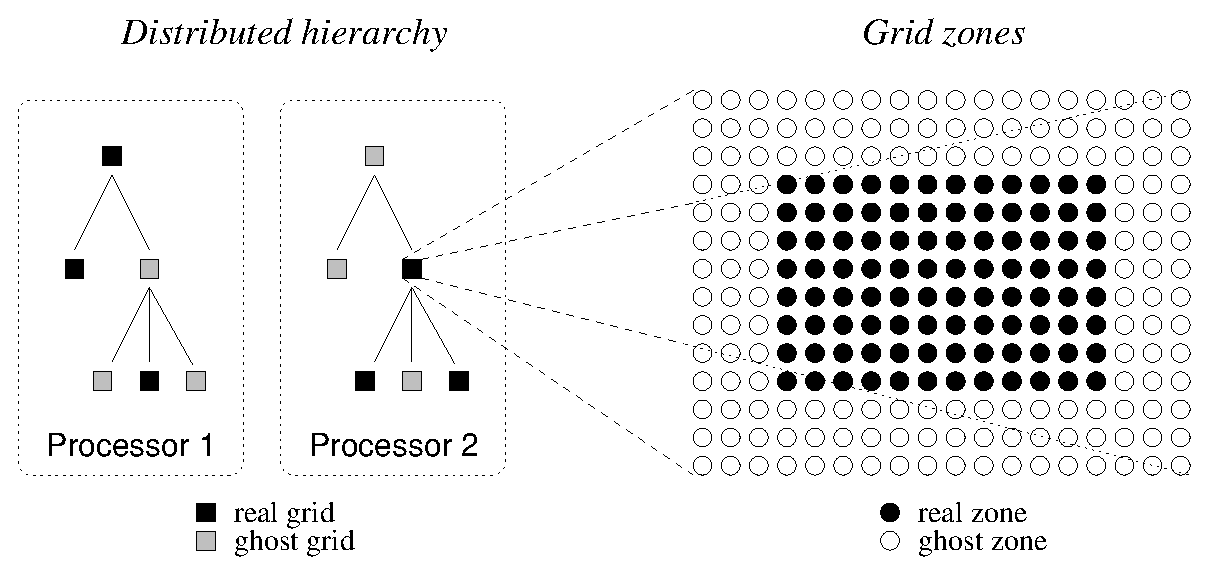
\includegraphics[width=0.4\textwidth]{figures/amr_hierarchy.eps}
\end{center}
\caption{\emph{Left:}  Example of a simple, 
distributed AMR hierarchy showing real and 
ghost grids.
\emph{Right:}  Example 2D \enzo\ grid showing real and ghost zones, as 
needed for the PPM hydro stencil.  Image courtesy of James Bordner (Cent.
Astrophysics and Space Sciences, UCSD).
}
\label{fig.2.amrhierarchy}
\end{figure}

\begin{figure}
\begin{center}
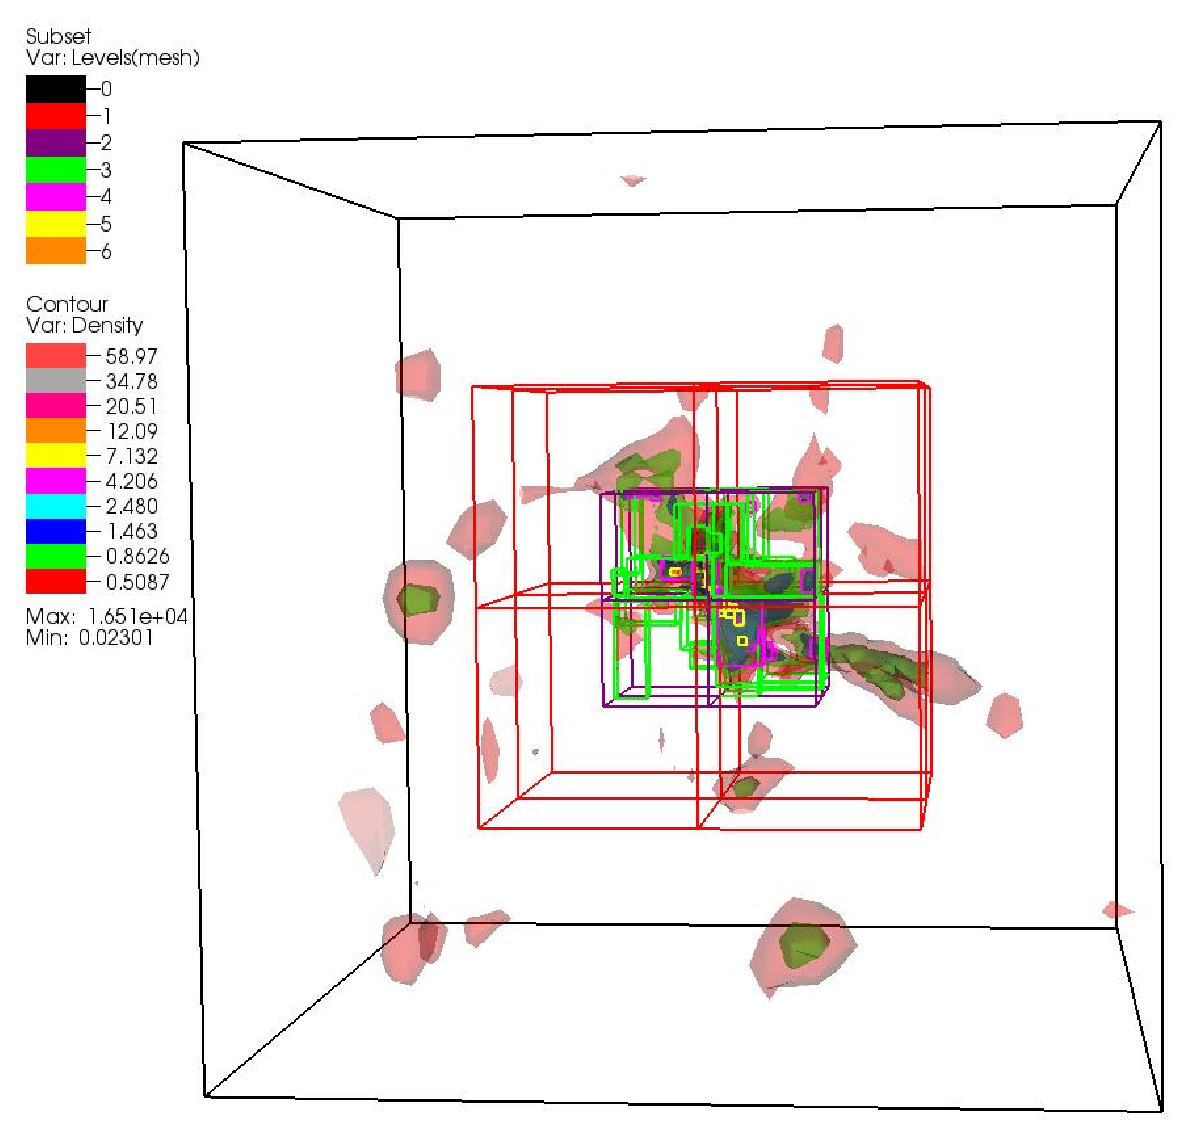
\includegraphics[width=0.4\textwidth]{figures/amr-hier-dens.eps}
\caption{Example of an \enzo\ simulation showing the AMR grid hierarchy.  
This is a simulation of the collapse of a single massive halo with a 
$32^3$ root grid and two $32^3$ static nested grids.  AMR is only allowed
within the most highly refined static nested grid.  Log baryon density is shown
by colored isocontours with values corresponding to the legend at center left.  
The rectangular solid wire frames correspond to individual 
AMR grids, with different colors corresponding to level as indicated by the
legend at top left.}
\label{fig.2.amrhierdens}
\end{center}
\end{figure}

Each grid patch in \enzo\ contains arrays of values for baryon and 
particle quantities.   Grids are 
partitioned into a core of \emph{real zones} and a surrounding layer 
of \emph{ghost zones}.  The real zones store field values and ghost 
zones are used to temporarily store values which have been obtained 
directly from neighboring grids or interpolated from a parent grid.  
These zones are necessary to accommodate the computational stencil of 
the hydrodynamics solvers (Sections~\ref{sec.ov.hydro.ppm} and~\ref{sec.ov.hydro.zeus}) 
and the gravity solver (Section~\ref{sec.ov.nbody}).  
The PPM and Zeus hydro solvers require 3 layers of ghost zones,  and the gravity
solver requires 6.  This can lead to significant memory 
and computational overhead, particularly for smaller grid patches
at high levels of refinement.  More information on filling of ghost
zones can be found in the appendix.

From the point of view of the hydro solver, each grid is solved as an
independent CFD problem, with Dirichlet boundary conditions stored in
the ghost zones.  At the end of each timestep, cells on a given level
fill ghost zones by interpolating from the parent and copying from
neighbors on the same level.  Grids then correct the flux at the interface boundary between
fine and coarse zones, and finally project their real zone data to the
parent grid. 

Timesteps are determined on each level as
described in \ref{sed.timestepping}, and the hierarchy is advanced on
a level by level basis in what's known as a W-Cycle.    Beginning with
the coarsest level, $L$, all grids on that level are advanced one
timestep.  Then one timestep is taken on all grids at the next level
of refinement, $L+1$, and so on until the finest level is resolved.
The finest level is then advanced, using as many steps as it takes to
reach the level immediately above.  The finest level is then synced
to the level above it, which then proceeds forewards one more step.
\red{Needs a picture of the W cycle.}

At the end of every timestep on every level each grid updates 
its ghost zones by exchanging information with its neighboring grid patches 
(if any exist) and/or by interpolating from a parent grid.  
In addition, cells are examined to see if they should be refined or 
de-refined, and the entire grid hierarchy is rebuilt at that 
level (including all more highly refined levels).  The timestepping and 
hierarchy advancement/rebuilding process described here is repeated 
recursively on every level to the specified maximum level of 
refinement in the simulation. 

Since the addition of more highly refined grids is adaptive,  
the conditions for refinement must be specified.  The criteria of 
refinement can be set by the threshold value of the overdensity of 
baryon gas or dark matter in a cell (which is really a refinement on
the mass of gas or DM in a cell), the local Jeans length, the 
local density gradient, or local pressure and energy gradients.  
A cell reaching any or all of these criteria 
will then be flagged for refinement.  
Once all cells at a given level have been examined, rectangular boundaries 
are determined which minimally encompass the flagged cells. The set of
flagging cells is then further fractured into smaller bounding
rectangles to ensure computational 
efficiency.  More details on subgrid creation can be found in Appendix
\ref{app.subgrid_creation}.  A refined grid patch is 
introduced within each such bounding rectangle. Thus the cells needing 
refinement, as well as adjacent cells within the patch which do not need 
refinement, are refined. While this approach is not as memory efficient as 
cell-splitting AMR schemes, it offers more freedom with 
finite difference stencils. For example, PPM requires a stencil of seven 
cells per dimension. This cannot easily be accommodated in cell-splitting 
AMR schemes. 

\blue{ \emph{I think this  should be
  re-written to reflect data presented or referenced in this paper,
  whatever that winds up being.}
In the simulations discussed in this thesis we typically use baryon and
dark matter overdensities as our refinement criteria, though
for some higher-resolution simulations we also refine on other
criteria as needed.} 

\subsection{Timestepping}\label{sec.timestepping}
\dcc{Made this its own section (not really part of the AMR, it's more
  general than that.)  Added stuff on harmonic average for 3d. See
  note below on acceleration timestep criterion being crap. Moved
  w-cycle to the previous section}
In \enzo, resolution of the equations being solved is adaptive in time 
as well as in space.  The timestep in \enzo\ is satisfied on a level-by-level
 basis by finding the largest timestep such that multiple criteria are
satisfied on each level.  The timestep criteria used by \enzo\ are 
(showing the one-dimensional case for clarity):

\begin{equation}
\Delta t_{hydro} = min \left( \kappa_{hydro} \frac{a \Delta x}{c_{s} + |v_x|} \right)_L ,
\label{eqn:dthydro}
\end{equation}

\begin{equation}
\Delta t_{dm} = min \left(\kappa_{dm} \frac{a \Delta x}{v_{dm,x}} \right)_L ,
\label{eqn:dtdarkmatter}
\end{equation}

\begin{equation}
\Delta t_{exp} = f_{exp} \left( \frac{a}{\dot{a}} \right) ,
\label{eqn:dtexpand}
\end{equation}

\begin{equation}
\Delta t_{accel} = min \left( \sqrt{\frac{\Delta x}{\myvec{g}}} \right)_L 
\label{eqn:dtaccel}
\end{equation}

 In equations~\ref{eqn:dthydro}-\ref{eqn:dtaccel}, the $min ( \ldots )_L$
formalism means that this value is calculated for all cells on a given level
L and the minimum overall value is taken as the timestep.  
Equation~\ref{eqn:dthydro} ensures that all cells satisfy the 
Courant-Freidrichs-Levy (CFL) condition for accuracy and stability of an explicit
finite difference discretization of the Euler equations.  Effectively this condition
forces the timestep to be small enough such that any changes in the fluid propagate
less than a single grid spacing, $\Delta x$.  In this equation, $\kappa_{hydro}$ is 
a numerical constant with a value of $0 < \kappa_{hydro} \leq 1$ (with a typical
value of $\kappa_{hydro} \sim 0.3-0.5$) that ensures that the CFL condition is always
met, and $c_s$ and $v_x$ are the sound speed and peculiar baryon
velocity in a given cell.

Equation~\ref{eqn:dtdarkmatter} is analogous to Equation~\ref{eqn:dthydro} and ensures
accuracy in the N-body solver by requiring that no dark matter particle travels more than
one cell width.  The parameter $\kappa_{dm}$ is analogous to $\kappa_{dthydro}$, with
an identical range of values.  Equation~\ref{eqn:dtexpand} limits the timestep such 
that the expansion parameter a can only change by a fractional amount of $f_{exp} = \Delta a/a$, 
where $f_{exp}$ is a user-defined parameter and has typical values of $f_{exp} = 0.01-0.02$.
This is required for the stability of the PPM algorithm in comoving coordinates, and
typically limits the timestep only at high redshifts when densities are relatively
homogeneous.

Equation~\ref{eqn:dtaccel} is supplementary to equation~\ref{eqn:dthydro} in that it
takes into account the possibility of large accelerations causing numerical 
instabilities by violating the Courant condition.  In this equation, $\myvec{g}$ is the
gravitational acceleration in each cell on level L.  \blue{ \emph{It should be
  noted that the timestep is computed before the acceleration field is computed,
  and the acceleration field is deleted at the end of each timestep.
  So this condition isn't ever actually enforced.  We should either
  fix this problem, or not discuss it.
 -dcollins.} }

Equation ~\ref{eqn:dthydro} is valid for one dimension.  For 2 or 3
dimensions, it was shown by \cite{Godunov1959}  that using the
harmonic average of the timestep found along each of the coordinate
axes yields a maximum $\kappa_{hydro} = 0.8$.  So letting $\Delta
t_x$, $\Delta t_y$, and $\Delta t_z$ be the analogues of
eqn. \ref{eqn:dthydro} along the $x,y$ and $z$ axes, 
\begin{equation}
\Delta t_{hydro} = min ( \kappa_{hydro} /( \frac{1}{\Delta t_x}
+\frac{1}{\Delta t_y} + \frac{1}{\Delta t_z} ) )_L
\end{equation}

For all other criteria, multiple dimensions are accounted for by
repeating the one dimensional criterion along each axis, and taking
the minimum.


%---------------------------------------------------------------------------%
\subsection{Parallelism}\label{sec.ov.parallel}
\dcc{moved hierarchy description, parallism notes from AMR section
  here. Mentioned performance/scaling study.  Still short.}

When \enzo\ is run on a distrubuted platform, some of the data is
replicated to all processors, while some remains on a single processor.
A description of the entire hierarchy (the position and size of each grid, as well
some other meta data) is stored on each processor.  This enables each
grid to know what grids are near it in the hierarchy, regardless of
where the data is.  The actual Baryon data (density, velocity, energy,
and any chemistry data) and particle data are stored on only one
processor.  Storing the entire hierarchy on all processor does create
some overhead, but in practice this is not an issue until one reaches
the extremely large scale.
  The code handles load balancing 
on a level-by-level basis such that the workload on each level is 
distributed as uniformly as possible across all processors.  Spatial locality of 
grids is not forced during message passing, for maximum flexibility (though not
necessarily maximum efficiency).  
The MPI message passing library\footnote{http://www-unix.mcs.anl.gov/mpi/}
 is used to transfer data between processors.

The performance of \enzo\ has been extensively studied using the
software package LCAPerf.  More on LCAPerf can be found in section
\ref{sec.performance} 

%old text
%Every processor 
%keeps a description of the entire grid hierarchy at all times, so that 
%each processor knows where all grids are.  However, baryon and particle 
%data for a given grid only exists on a single processor.  See 
%Figure~\ref{fig.2.amrhierarchy} for a schematic example of this.  


%%% Local Variables: 
%%% mode: latex
%%% TeX-master: "ms"
%%% End: 
